\documentclass[11pt]{article}
\usepackage[utf8]{inputenc}	% Para caracteres en español
\usepackage{amsmath,amsthm,amsfonts,amssymb,amscd}
\usepackage{multirow,booktabs}
\usepackage[table]{xcolor}
\usepackage{fullpage}
\usepackage[bottom]{footmisc}
\usepackage{lastpage}
\usepackage{enumitem}
\usepackage{fancyhdr}

\usepackage{mathrsfs}
\usepackage{wrapfig}
\usepackage{setspace}
\usepackage{calc}
\usepackage{multicol}
\usepackage{cancel}
\usepackage[retainorgcmds]{IEEEtrantools}
\usepackage[margin=3cm]{geometry}
\usepackage{amsmath}
\usepackage{algorithm}
\usepackage{algpseudocode}
\newlength{\tabcont}
\setlength{\parindent}{0.0in}
\setlength{\parskip}{0.05in}
\usepackage{empheq}
\usepackage{framed}
\usepackage[most]{tcolorbox}
\usepackage{xcolor}
\colorlet{shadecolor}{orange!15}
\parindent 0in
\parskip 12pt
\geometry{margin=1in, headsep=0.25in}
\theoremstyle{definition}
\newtheorem{definition}{Definition}
\newtcbtheorem[auto counter,number within=section]{theorem}%
  {Theorem}{fonttitle=\bfseries\upshape, fontupper=\slshape,
     arc=0mm, colback=blue!5!white,colframe=red!75!black}{defn}

\newtcbtheorem[auto counter,number within=section]{defn}%
    {Definition}{fonttitle=\bfseries\upshape, fontupper=\slshape,
    arc=0mm, colback=blue!5!white,colframe=green!75!black}{defn}

\newtheorem{reg}{Rule}
\newtcbtheorem[auto counter,number within=section]{proposition}%
{Proposition}{fonttitle=\bfseries\upshape, fontupper=\slshape,
    arc=0mm, colback=blue!5!white,colframe=blue!75!black}{proposition}
\newtcbtheorem[auto counter,number within=section]{lemma}%
{Lemma}{fonttitle=\bfseries\upshape, fontupper=\slshape,
    arc=0mm, colback=blue!5!white,colframe=yellow!75!black}{lemma}
    
\newtheorem{exer}{Exercise}
\numberwithin{equation}{section}

\numberwithin{definition}{section}
\usepackage{hyperref}
\usepackage{xurl}
\usepackage{listings}
\usepackage{subcaption}
\title{Popular Erasmus destinations}
\author{Alessandro Lotta, Youssef Ben Khalifa}
\date{\today}
\begin{document}
\maketitle \tableofcontents 
\newpage

\section{Dataset creation and pre-processing}
To manage the large amount of data we had to work with, we decided to make use of a custom created class called \textbf{Dataset}, in which we define all the 
methods and objects we used. 

The dataset class makes use of the \textbf{pandas} library, which is a Python library for data manipulation and analysis, with which 
we perform the import, the preprocessing and the manipulation of the datasets. 
\subsection*{Dataset creation}
As mentioned in the other reports, the dataset was extracted from a list of .csv files (the source can be found in the references section), from which 
we selected all the data going from 2014 to 2019. The dataset is then loaded into a single Pandas Dataframe object, from which we will then further 
filter out and clear the data we do not need. 

\subsection*{Dataset preprocessing}
The first thing we need to do is to clear out the entries that are either incomplete or not useful for our analysis. To do that, 
we start by applying a simple filter on the dataset to select only the columns we are interested in, to then remove all 
the rows that have at least one missing value. This is done using the \textit{cleanDataframe()} method contained in the dataset class. 

From the resulting dataset we can start to filter out the type of entries we need for each of our analysis using the \textit{applyFilter()} method: 
for our analysis we kept the entries associated to only the students that were still going through either a bachelor or a master degree in the respective
university.

\section{Graph creation}
The entire project is based on the usage of the python library \textbf{NetworkX} which is a Python library for the creation, manipulation and study of the structure, dynamics, and functions of complex networks.

Originally, we meant to use a dedicated class called \textit{CustomGraph}, which can be found in the \textit{graph.py} file, to manage the graph
and its entries, but this method revealed itself to be quite time consumnig and computationally heavy. So we then opted to adopt a 
dedicated function found in the NetworkX library that allowed us to create the graph with all its nodes and edges by simply feeding the method 
a dataframe object in which we specify, for each edge, the starting and end node, along with the weight of the edge. 
\\
The \textit{weight} of an edge in our graphs is determined by the total amount of students that participated in the Erasmus program in which the Sending and Receiving 
country/university are respectively the starting node and ending node associated with that edge.
The graph creation was achieved using the following code:
\begin{lstlisting}[caption={Country Graph creation}, language=python]
import networkx as nx
import pandas as pd
edges = pd.DataFrame({"source" : ds.df["Sending Country Code"],
                      "target" : ds.df["Receiving Country Code"],
                      "weight" : ds.df["Participants"]
                         })
edges = edges.groupby(['source', 'target']).sum().reset_index()
CountryGraph = nx.from_pandas_edgelist(edges, "source", "target", "weight", nx.DiGraph())
\end{lstlisting}
The same process was done to create both the graph containing the countries as nodes and the one with the universities.

At the end we end up with two graphs onto which wee can perform our analysis, each with the following dimensions:

\begin{table}[!ht]
  \centering
  \begin{tabular}{l|ll}
  \rowcolor[HTML]{FFFFFF} 
  \textbf{Dimensions} & \textbf{CountryGraph} & \textbf{UniGraph} \\ \hline
  \textit{\# Nodes}   & 152                   & 76816             \\
  \textit{\# Edges}   & 3420                  & 185126           
  \end{tabular}
  \end{table}


\section{Analysis performed}
    In this section we will go over all the analysis we have performed on the graph we generated from the data we had.
    As we said in the project proposal we will use two graphs $C = (V_c, E_c)$ and $U = (V_u, E_u)$: 
    one having countries as nodes and the other one having universities as nodes, 
    in which the edges and their weights represent the amount of students moving/received from one node to the other.

    \subsection*{PageRank coefficient}

    The \textbf{PageRank} coefficient of a node $v$ expresses the "importance" of a node in the graph, this is done by considering the 
    number of incoming edges and the PageRank coefficient of the nodes that are connected to it. Analytically, the PageRank coefficient of a node $v$ is defined as:
    \begin{equation}
        Pr(v) = (1-d) + d \sum_{u \in V} \frac{Pr(u)}{deg(u)}
    \end{equation}
    where $d$ is the \textbf{damping factor} given by the user, $V$ is the set of nodes in the graph and $deg(u)$ is the degree of node $u$.
    \\\\
    This particular feature is very useful when we compute it on the graph in which we define as the set of nodes and edges, respectively the 
    countries/universities and as edges both the students that are sent and received. We can find a measure of how important a country or a 
    university can be in terms of students flow.
    \subsubsection*{PageRank coefficient implementation}
    We implemented the PageRank algorithm using the \textbf{NetworkX} library, using the following method:
    \begin{lstlisting}[language=python]
      _ranks = nx.pagerank(CountryGraph, weight='weight')
    \end{lstlisting}

    \subsection*{HITS}
    The Hyperlink-Induced Topic Search (HITS) is a link analysis algorithm that rates nodes based on two scores, 
    a hub score and an authority score. The authority score estimates the importance of the node within the network. 
    The hub score estimates the value of its relationships to other nodes. 
    The GDS implementation is based on the Authoritative Sources in a Hyperlinked Environment publication by Jon M. Kleinberg.
    \subsubsection*{HITS implementation}
    NetworkX also provides the method for computing the HIST score for a given graph:
    \begin{lstlisting}[language=python]
      (hubs, authorities) = nx.hits(CountryGraph)
    \end{lstlisting}

    \section{Analysis results and comparisons}
    Each analysis was done on two different machines in order to try and extrapolate a measure of the efficiency of the algorithms we used. 
    However, the comparisons between the different time results on the algorithm execution are not very reliable, since the machines used
    are affected by many other factors other that the hardware itself. 

    The main focus of the analysis is on how the algorithms implementations we adopted perform w.r.t. the size of the graph we created.

    To analyze and compare the results we decided to concentrate only on the Students that participate on the Erasums program while being
    subscribed to a Master Degree, to do this we applied a filter on the "Education Level" column selecting the value "ISCED-7".
    \subsection*{Compution time results and comparisons}
    For the test we had at our disposal two different machines:
    \begin{enumerate}
      \item Asus ROG laptop with an AMD Ryzen 9 5900HS CPU @ 3.00->4.6 GHz, Nvidia RTX 3060 (Mobile) Dedicated GPU, 16GB of RAM;
      \item ----------------PC ALE -----------------;
    \end{enumerate}
    the results are computed separately for both graphs:

  \begin{table}[!ht]
    \centering
    \begin{tabular}{l|ll}
    \rowcolor[HTML]{FFFFFF} 
    \textbf{Algorithm}            & \textbf{Asus ROG}   & \textbf{--- PC ALE ----} \\ \hline
    \textit{PageRank}             & 0.01854991912841797 & ----------               \\
    \textit{Hits}                 & 0.1143503189086914  & ------------             \\
    \end{tabular}
    \caption{Results for CountryGraph}
  \end{table}
  \begin{table}[!ht]
    \centering
    \begin{tabular}{l|ll}
    \rowcolor[HTML]{FFFFFF} 
    \textbf{Algorithm}            & \textbf{Asus ROG}   & \textbf{--- PC ALE ----} \\ \hline
    \textit{PageRank}             & 2.0881154537200928 & ----------               \\
    \textit{Hits}                 & 2.626953125  & ------------             \\
    \end{tabular}
    \caption{Results for UniGraph}
  \end{table}

  Considering the difference in dimensions between the two graphs, the algorithm manages to obtained 
  good results on the UniGraph compared to the CountryGraph. Again, the reliability of the results cannot 
  bee guaranteed as there are to many factors that can affect the performance of the machines.

    \subsection*{Countries Results}
    The results obtained are presented by showing the top countries based on the values obtained from PageRank and HITS.
    \begin{table}[hbtp]
        \parbox{.25\linewidth}{
        \centering
        \begin{tabular}{l l}
            \hline
            \textbf{Country} & \textbf{PageRank} \\ \hline
            France & 5.719243 \\
            Italy & 4.760962 \\
            Germany & 4.507946 \\
            Tunisia & 4.419083 \\
            Spain & 4.150749 \\\hline
          \end{tabular}
          \label{tab:table-label}
        }
        \hfill
        \parbox{.25\linewidth}{
        \centering
        \begin{tabular}{l l}
            \hline
            \textbf{Country} & \textbf{Authorities} \\ \hline
            France & 9.997428 \\
            Italy & 5.675233 \\
            Germany & 3.920258 \\
            Spain & 1.839538 \\
            Poland & 1.600657 \\ \hline
          \end{tabular}
          \label{tab:table-label}
        }
        \hfill
        \parbox{.25\linewidth}{
        \centering
        \begin{tabular}{l l}
            \hline
            \textbf{Country} & \textbf{Hubs} \\ \hline
            Tunisia & 11.644793 \\
            Vietnam & 3.165710 \\
            Algeria & 2.065967 \\
            Egypt & 1.954555 \\
            Montenegro & 1.025746 \\ \hline
          \end{tabular}
          \label{tab:table-label}
        }
        \end{table}
    
    For the country graphs we also decided to implement the code to generate the geographical heatmaps by using the library
    'geopandas', so that we can obtain more representative results.
    The geographical maps were created by only considering Europe and excluding the country Russia.
    An example of these is the following map obtained with the PageRank results

    \begin{figure}[H]
        \centering
          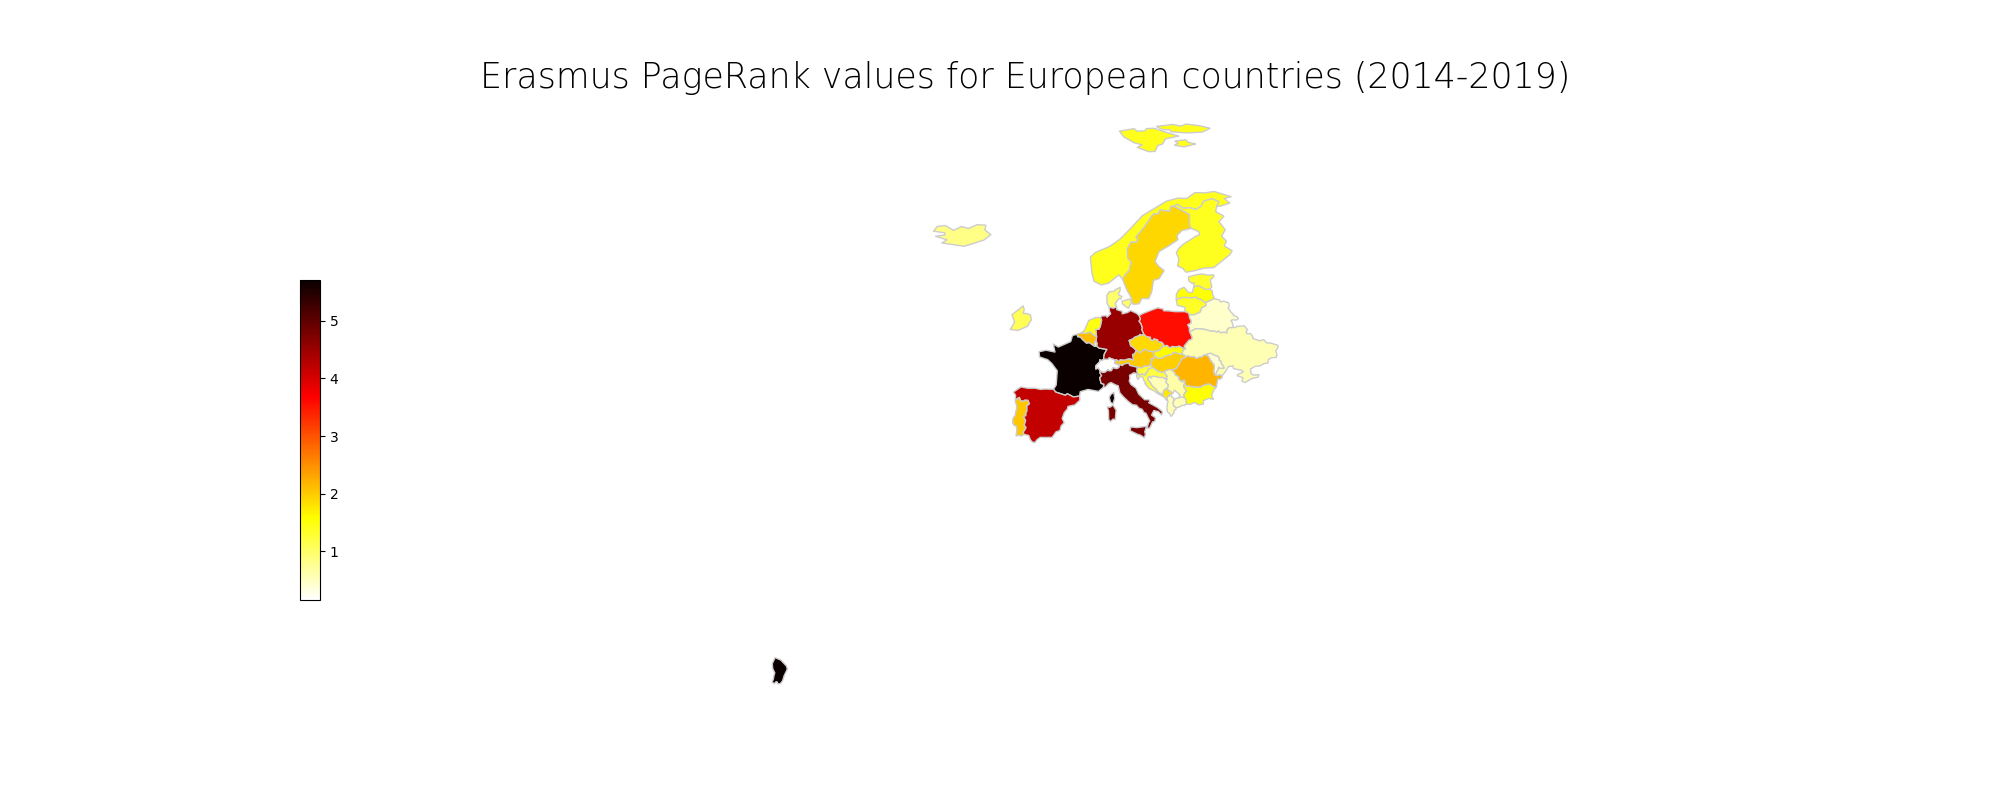
\includegraphics[width=\linewidth]{../geoMaps/PR_geoMap.png}
          \caption{PageRank Heatmap}
         \label{fig:1}
        \end{figure}     

    From the results we obtained it is possible to see that there are some differences between the two methods,
    more in detail in the top results for PageRank and Authorities values there are almost the same countries(France,Italy,Germany,Spain)
     instead the Hubs values are completely different.
    
    Finally heare are the top 5 contries by centrality score:

    \subsection*{Universities Results}
    In the case of the results obtained with the UniNodes graph, we can observe that the PageRank and Hits values 
    have different rankings for top Universities, except for "UNIVERSIDADE DE LISBOA" which is the most important
    for both PageRank and Authorities.
    From the table containing the Hubs scores it is clear that the most relevant Universities in Italy are also the 
    ones that have students traveling to the universities that have high Authorities values. 
    In particular "UNIVERSITA DEGLI STUDI DI ROMA" and "POLITECNICO DI MILANO" have also the top PageRank values.    
    \begin{table}[hbtp]
      \parbox{.25\linewidth}{
        \centering
        \begin{tabular}{l l}
            \hline
            \textbf{Organization} & \textbf{PageRank} \\ \hline
            UNIVERSIDADE DE LISBOA & 49.156703 \\
            Stichting ArtEZ & 45.381767 \\
            UNIVERSITA DEGLI STUDI DI ROMA LA SAPIENZA & 44.403827 \\
            Eesti Kunstiakadeemia & 42.335885 \\
            POLITECNICO DI MILANO & 41.404278\\\hline
          \end{tabular}
          \label{tab:table-label}
        }
      \end{table}

    \begin{table}[hbtp]
        \parbox{.25\linewidth}{
        \centering
        \begin{tabular}{l l}
            \hline
            \textbf{Organization} & \textbf{Authorities} \\ \hline
            UNIVERSIDADE DE LISBOA & 8.715438e+01 \\
            NORGES TEKNISK-NATURVITENSKAPELIGE UNIVERSITET.. & 6.628848e+01 \\
            UNIVERSITAT POLITECNICA DE CATALUNYA & 6.617643e+01 \\
            UNIVERSITAT POLITECNICA DE VALENCIA & 6.022172e+01 \\
            KATHOLIEKE UNIVERSITEIT LEUVEN & 5.544156e+01 \\ \hline
          \end{tabular}
          \label{tab:table-label}
        }
        \end{table}
        \begin{table}[H]
        \parbox{.25\linewidth}{
        \centering
        \begin{tabular}{l l}
            \hline
            \textbf{Organization} & \textbf{Hubs} \\ \hline
            ALMA MATER STUDIORUM - UNIVERSITA DI BOLOGNA & 9.454380e+01 \\
            UNIVERSITA DEGLI STUDI DI PADOVA & 7.960611e+01 \\
            UNIVERSITA DEGLI STUDI DI ROMA LA SAPIENZA & 7.632965e+01 \\
            POLITECNICO DI MILANO & 7.479510e+01 \\
            UNIVERSIDADE DE LISBOA & 6.127300e+01 \\ \hline
          \end{tabular}
          \label{tab:table-label}
        }
        \end{table}
    
        Then as we did with the CountryGraph, we computed the centrality score for the universities graph:

    \section{Further analysis and improvements}
    \begin{enumerate}
        \item Use of the \textbf{Random graphs} method to verify if the features we extracted actually give out interesting information;
        \item Compute the same score on different types of graphs using different filters on the orinating dataset. 
        \item Try and obtain more recent data and repeat the analysis.
    \end{enumerate} 
  
    \section{Team Effort}
    We are listed the contribution of each member of the team and the duration of each stage of the project:
    \begin{itemize}
      \item \textbf{Dataset Creation} : Youssef Ben Khalifa [2h], 
      \item \textbf{Dataset Preprocessing and Filtering} : Youssef Ben Khalifa [1.5h], 
      \item \textbf{Grah creation} : Youssef Ben Khalifa [3h],
      \item \textbf{PageRank computation} : Youssef Ben Khalifa [1h],
      \item \textbf{HITS computation} : 
      \item \textbf{Results visualization} : Youssef Ben Khalifa [1h]
    \end{itemize}
  \section{References}
    \begin{itemize}
        \item The official portal for European data. \textit{Erasmus mobility statistics 2014 - 2019}. \url{https://data.europa.eu/data/datasets/erasmus-mobility-statistics-2014-2019-v2?locale=en} 
        \item NetworkX - Network Analysis in Python. \textit{PageRank algorithm documentation}. \url{https://networkx.org/documentation/stable/reference/algorithms/generated/networkx.algorithms.link_analysis.pagerank_alg.pagerank.html}
        \item NetworkX - Network Analysis in Python. \textit{HITS algorithm documentation}. \url{https://networkx.org/documentation/stable/reference/algorithms/generated/networkx.algorithms.link_analysis.hits_alg.hits.html}
    \end{itemize}
    \end{document}